% Plantilla realizada por Alberto Brunete (UPM).

%Parametros de tipo libro
\documentclass[10pt,a4paper]{book}

%Idioma español y acentos
\usepackage[spanish, es-tabla]{babel}
%\usepackage[latin1]{inputenc}
\usepackage[utf8]{inputenc}

%algunos sÌmbolos matemáticos y paquetes para usar subimágenes
\usepackage{amsmath}
\usepackage{amsfonts}
\usepackage{amssymb}
\usepackage{graphicx}
\usepackage{subfigure}
\usepackage{listings}
\usepackage{appendix}
%Márgenes
\usepackage[left=3cm,top=3cm,right=3cm,bottom=3cm]{geometry}

%
\usepackage{multicol}

%para generar índice con hipervínculos
\usepackage{hyperref}

%parametros del documento (sus propiedades)
\hypersetup{
    pdftitle={Nombre del alumno - TFG - año},
    pdfsubject={TFG - año},
    pdfauthor={Nombre del alumno},
    pdfkeywords={palabraclave1} {palabraclave2} {palabraclave3},
    colorlinks,
    citecolor=black,
    filecolor=black,
    linkcolor=black,
    urlcolor=black,
}

%Código
\usepackage{listings}
%Rename Listlings
\renewcommand{\lstlistingname}{Código}% Listing -> Algorithm
\renewcommand{\lstlistlistingname}{Lista de \lstlistingname s}
% List of Listings -> Lista de Código

%empieza el documento
\begin{document}  

%elementos antes del trabajo en sÌ se meten dentro de frontmatter
\frontmatter

%cada incluye referencia a un archivo de tipo .tex
\begin{titlepage}
\begin{center}

%forma de introducir imágenes. el \\[0.5 cm] de final de línea introduce un salto de ese tamaño.
%width=1\textwidth indica el tamaño de la imágen (valores entre 0-1). 
 
\includegraphics[width=1\textwidth]{figuras/cabecera.png}  \\[0.5 cm]

\LARGE UNIVERSIDAD POLITÉCNICA DE MADRID \\ [1 cm]

\LARGE ESCUELA TÉCNICA SUPERIOR DE INGENIERÍA Y DISEÑO INDUSTRIAL \\ [1 cm]

\LARGE Grado en Ingeniería Electrónica y Automática Industrial\\ [1 cm]

\LARGE \textbf{TRABAJO FIN DE GRADO}\\[1 cm]

\Huge \textsc{Título del trabajo}\\[1 cm]

\LARGE Autor \\[2 cm]

%flushleft alinea a la izquierda el texto

\begin{multicols}{2} 
\begin{flushleft} \Large
\emph{Cotutor (si lo hay):} nombre y apellidos \\
\emph{Departamento:} departamento
\end{flushleft}

\begin{flushleft} \Large
\emph{Tutor:} nombre y apellidos\\
\emph{Departamento:} departamento
\end{flushleft}

\end{multicols} 

%rellena de blanco el resto de la página para escribir abajo del todo
\vfill

% Bottom of the page
{\large Ciudad, Mes, Año}

%SE ponen al final firmas.tex
%\end{center}
%\end{titlepage}


\cleardoublepage 

%\begin{center}
% Está puesto en portada.tex
\thispagestyle{empty}
%forma de introducir imágenes. el \\[0.5 cm] de final de línea introduce un salto de ese tamaño.
%width=1\textwidth indica el tamaño de la imágen (valores entre 0-1). 

\includegraphics[width=1\textwidth]{figuras/cabecera.png}  \\[0.5 cm]

\LARGE UNIVERSIDAD POLITÉCNICA DE MADRID \\ [1 cm]

\LARGE ESCUELA TÉCNICA SUPERIOR DE INGENIERÍA Y DISEÑO INDUSTRIAL \\ [1 cm]

\LARGE Grado en Ingeniería Electrónica y Automática Industrial\\ [1 cm]

\LARGE \textbf{TRABAJO FIN DE GRADO}\\[1 cm]

\Huge \textsc{Conexion de RoboHealthArm a una red domotica empleando radiofrecuencia}\\[2 cm]

\Large Firma Autor \\[3 cm]

%flushleft alinea a la izquierda el texto

\begin{multicols}{2} 
\begin{flushleft} 
\Large \emph{Firma Cotutor (si lo hay)}
\end{flushleft}

\begin{flushright} 
\Large \emph{Firma Tutor}
\end{flushright}

\end{multicols} 

%rellena de blanco el resto de la página para escribir abajo del todo
\vfill

\end{center}
\end{titlepage}


\cleardoublepage 

%Licencia opcional
\begin{flushleft}

Copyright \copyright  2019. José Luis Grande Morón.

%ejemplo de licencia, se puede elegir cualquier otra

Esta obra está licenciada bajo la licencia Creative Commons Atribución-NoComercial-SinDerivadas 3.0 Unported (CC BY-NC-ND 3.0). Para ver una copia de esta licencia, visite http://creativecommons.org/licenses/by-nc-nd/3.0/deed.es o envíe una carta a Creative Commons, 444 Castro Street, Suite 900, Mountain View, California, 94041, EE.UU.

Todas las opiniones aquí expresadas son del autor, y no reflejan necesariamente las opiniones
de la Universidad Politécnica de Madrid.

\end{flushleft}

\cleardoublepage

\begin{flushleft} \large
\textbf{Titulo:} Conexión de RoboHealthArm a una red domótica empleando radiofrecuencia \\
\textbf{Autor:} José Luis Grande Morón\\
\textbf{Tutor:} Alberto Brunete González \\  [1 cm]

\end{flushleft} 

\begin{center} \LARGE
EL TRIBUNAL \\ [1 cm]
\end{center}

\begin{flushleft} \LARGE
Presidente: \\ [1 cm]
Vocal: \\ [1 cm]
Secretario: \\ [1.5 cm]
\end{flushleft}

\large
Realizado el acto de defensa y lectura del Trabajo Fin de Grado el día ....... de ....................   de ... en .........., en la Escuela Técnica Superior de Ingeniería y Diseño Industrial de la Universidad Politécnica de Madrid, acuerda otorgarle la CALIFICACIÓN de: \\ [2 cm]

\begin{center}
 \large VOCAL \\ [2.2 cm]
\end{center}

\begin{minipage}{0.5\textwidth}
 \begin{flushleft}
 \large SECRETARIO
\end{flushleft}
\end{minipage}
\begin{minipage}{0.5\textwidth}
\begin{flushright}
 \large PRESIDENTE
\end{flushright} 
\end{minipage}

\chapter{Agradecimientos}

A mis abuelos. María, Sofía, Mariano y José. De todos ellos tengo algo que me ha ayudado durante estos años y que, no tengo duda, seguirá ayudándome. El valor del trabajo, el esfuerzo y el conocimiento.

A mis padres y a mi hermana.

A mis compañeros y sus consecuencias.

A Irene.

A todos ellos, muchas gracias por todo.

%chapter introduce un nuevo capítulo
\chapter{Resumen}

El presente proyecto se resume en el desarrollo de un sistema de comunicación usando radiofrecuencia que permita la integración del brazo robótico \textit{RoboHealth Arm} en la red de control de dispositivos actualmente disponible. El objetivo es mejorar la capacidad actual del brazo robótico para proporcionar asistencia a un supuesto paciente en un entorno hospitalario, función para la que fue diseñado.

\paragraph{Palabras clave:} Xbee, Node-RED, MQTT, radiofrecuencia, robótica.


\chapter{Abstract}

This document aim is to describe the development of a communication system based on radiofrequency to allow the complete integration of a robotic arm into an available domotic net. The main objetive is to improve the arm capacities in order to provide a better assistance to pacients in hospitals, as it was the reason why it was designed.

\paragraph{Keywords:} Xbee, Node-RED, MQTT, radiofrequency, robotics.

%genera índice
\tableofcontents
\addcontentsline{toc}{chapter}{Índice}

%Índice de figuras.
\listoffigures

%Índice de tablas.
\listoftables


%Empieza la parte descriptiva del trabajo
\mainmatter

\chapter{Introducción}

El presente documento corresponde a la realización de un Trabajo Final del Grado en Electrónica Industrial y Automática basado en la conexión e integración de un brazo robótico en una red domótica. A continuación, se recoge de manera ordenada y detallada el desarrollo e implementación del proyecto; así como los resultados obtenidos y las conclusiones a kas que es posible llegar.

\section{Motivación del proyecto}

El punto de partida es el proyecto Robohealth. Consiste en un conjunto de entidades en colaboración para el desarrollo de soluciones relacionadas con la robótica y la domótica con el fin de introducir mejoras en el sistema sanitario. Como se puede observar, entre estas entidades está, además de otras dos universidades públicas de la Comunidad de Madrid, la Universidad Politécnica de Madrid.

Los resultados del proyecto están orientados a pacientes con enfermedades crónicas o capacidades cognitivas limitadas, pacientes en una situación de dependencia a los que es posible mejorar la calidad de vida. Estas mejoras se obtienen a través del diseño y fabricación de robots de asistencia, tanto para pacientes como para sus cuidadores, y la implementación de entornos inteligentes.

En la figura \ref{fig:RH}, se pueden observar los diferentes paquetes de trabajo y subproyectos en los que se trabaja dentro de la estructura de RoboHealth, repartidos entre las entidades colaboradoras. En la Universidad Politécnica de Madrid, encargada del desarrollo de entornos inteligentes de asistencia y rehabilitación, se ha venido trabajando en distintas herramientas enmarcadas en Trabajos Finales de Grado durante los últimos años.

\begin{figure}[tb]
\centering
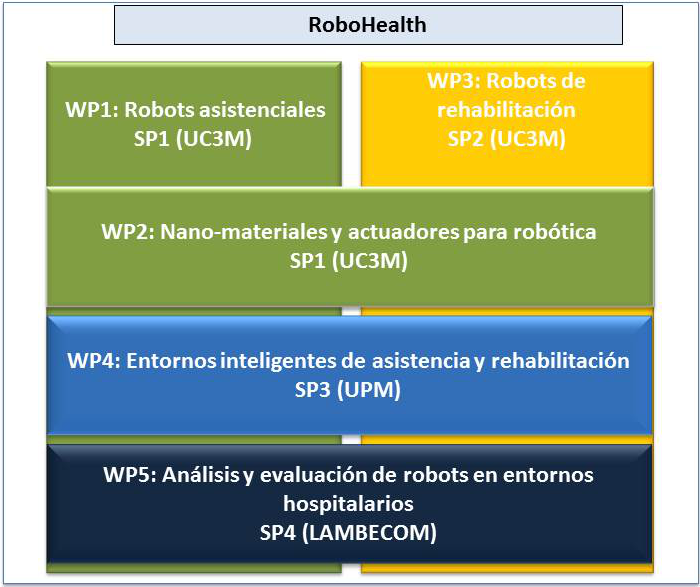
\includegraphics[width=0.55\textwidth]{figuras/RHstruct.png}
\caption{Estructura RoboHealth}
\label{fig:RH}
\end{figure}

Dentro del marco previamente expuesto, se han desarrollado dos plataformas que sirven de base para el proyecto objetivo de este documento.

\begin{itemize}
\item \textbf{RoboHealth Arm} es un brazo robótico de tres grados de libertad (actualmente, cuenta con sólo dos grados de libertad operativos) diseñado para sustentar una tablet en su extremo, haciendo más acesible su uso para pacientes y cuidadores. Está basado en un sitema de cuerdas y poleas accionado por tres servomotores.
\item Por otro lado, existe una aplicacion de \textbf{Node-RED} que integra los diferentes dispositivos y proyectos desarrollados en una red domótica. Incluye una interfaz gráfica que facilita su interacción vía internet, posibilitando controlar los dispositivos desde cualquier lugar.
\end{itemize} 

La idea es continuar el proceso de integración de los diferentes dispositivos en Node-RED con la intención de controlar todo desde la misma interfaz. En ese contexto, surge el proyecto de hacerlo con el brazo RoboHealth Arm. Con el fin de tratar de explorar todas las tecnologías posibles, se comprueba que la radiofrecuencia aún no habia sido y existen soluciones económicas en el mercado.

Así, el planteamient del Trabajo Final de Grado tomó forma, defiendose como la conexión mediante el uso de radiofrecuencia del brazo RoboHealth Arm a la interfaz de Node-RED. Para la radiofrecuencia, se usarán dispositivos XBee.

\section{Objetivos}

El fin del proyecto es la completa integración de un control a través de internet del brazo robótico. Los comandos se lanzan desde la interfaz de Node-Red y el ordenador de la sala transmite la orden vía radiofrecuencia al brazo.

Se ha desarrollado a posibilidad de configurar las coordenadas articulares del brazo antes de ser enviadas, dentro de su rango óptimo de trabajo actual.

La orden de Node-Red pone en marcha la ejecución de un script en Python que toma esos parámetros previamente especificados y envía por uno de los puertos serie el correspondiente frame. Este frame está pensado de acuerdo a las especificaciones de comunicación del brazo y del encapsulamiento de las comunicaciones de radio.

Un dispositivo XBee ha sido configurado para enviar el frame de datos recibido por comunicación serial. Al poder concentrarse todo el procesamiento de la información correspondiente al emisor en el anteriormente mencionado script, no se precisa de ningún microcontrolador adicional que funcione junto al módulo de radiofrecuencia. Así pues, el módulo XBee funciona de manera exclusiva como un traductor entre la información en el puerto serie correspondiente y las ondas de radiofrecuencia.

El dispositivo XBee receptor de la información que comanda el brazo robótico esta situado en el mismo. Su objetivo es ser capaz de captar el mensaje de radio específicamente diseñado para él y transmitirlo al microcontrolador del brazo. De la misma manera que en el otro XBee, su función será la de traductor de las ondas de radio (excusivamente de las destinadas a él) en información en el puerto serial. Esto es posible gracias al prediseño de los frames de información de acuerdo a las especificaciones y protocolos de comunicación del brazo.

El dispositivo operativo provoca la reacción esperada en el brazo, moviendo sus servos hasta las coordenadas articulares especificadas.

\section{Materiales utilizados}

Aquí se pueden citar todos los materiales utilizados, tanto software como hardware, para que el lector tenga una primera de lo que se va a hablar en el TFG.

\subsection{Componentes hardware}

\subsection{Componentes software}

\section{Estructura del documento}

A continuación y para facilitar la lectura del documento, se detalla el contenido de cada capítulo.

\begin{itemize}
\item En el capítulo 1 se realiza una introducción.
\item En el capítulo 2 se hace un repaso...
\end{itemize}

  
  %partes finales del trabajo: conclusiones, bibliografia y anexos

\chapter{Marco Teórico}

En este capítulo se describen (brevemente) todos los conceptos necesarios para entender el trabajo. No se trata de copiar el contenido de los libros de texto, si no de hacer un resumen de los conceptos necesarios para facilitar la lectura del documento al lector. Se entiende que el lector de un TFG tiene que tener unos conocimientos mínimos sobre el tema.
  
\chapter{Estado del arte}

A continuación, se hace un repaso de la tecnología existente en la actualidad relacionada con los campos tocados por el presente proyecto. El objetivo es proporcionar al lector un punto de partida del trabajo y comentar las soluciones utilizadas por otros autores. 

\section{Water level control using Raspberry Pi + XBee + XBMQ + MQTT + Node-Red \cite{zhivazhiva:RaspberryPi}}

Se trata de un proyecto que trabaja de manera bastante similar al trabajo objetivo del presente documento, teniendo ciertas tecnologías en común.

El objetivo es el control de una pequeña bomba de agua que llena un depósito lentamente, con una distancia considerable entre ambos elementos y el ordenador central. La motivación para automatizar el proceso de llenado del depósito era evitar ciertos incidentes provocados por el olvido de la persona que controlaba la bomba, debido a los extensos tiempos que se tomaba el sistema para llenar el depósito. El autor comenta que la señal se perdía frecuentemente al usar unos módulos Wi-Fi baratos y terminó decidiéndose por la tecnología XBee de Digi, descartando cualquier tecnología que no fuera inalámbrica por los motivos de distancia comentados previamente.

\begin{figure}[tb]
\centering
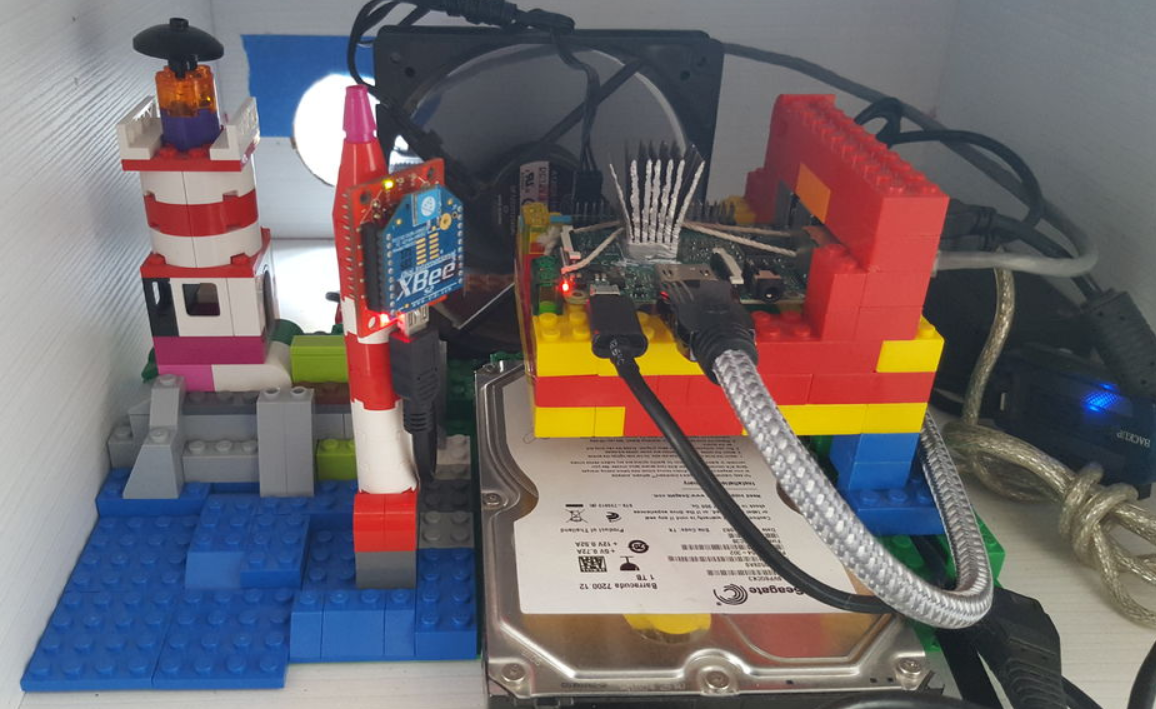
\includegraphics[width=0.55\textwidth]{figuras/EArte1.png}
\caption{Montaje del proyecto 3.1}
\label{fig:EArte1}
\end{figure}

Una Raspberry Pi3 ejerce de ordenador central del sistema y es el componente encargado de coordinar la interacción con el usuario que manda la orden y la interacción con el depósito y la bomba de agua vía XBee (montaje en la figura \ref{fig:EArte1}).

\begin{itemize}
\item Por un lado, tiene instalado Mosquitto (MQTT); un programa que usa la red para crear una especie de "tablón de anuncios" virtual. Los dispositivos conectados a esa red pueden suscribirse a un \textit{topic} y recibir lo que otros dispositivos publican en él.
La idea es que, haciendo uso de diferentes aplicaciones (como puede ser el caso de \textit{IoT MQTT Dashboard} en Android), se puedan publicar ciertos mensajes en algún \textit{topic} al que esté suscrita la Raspberry Pi desde otros dispositivos de manera remota. La Raspberry recibe esta información y actúa en consecuencia.
\item XBMQ actúa de puente dentro de la Raspberry Pi entre MQTT y el módulo XBee conectado a la misma, que es el que se comunica con el actuador y el sensor.
\item La Raspberry Pi envía los comandos al actuador y recibe la información del sensor a través del módulo XBee. En el lado del depósito, se sitúa el otro XBee con una salida controlando un pequeño relé que acciona y desactiva la bomba y una entrada que envía al XBee de la Raspberry el estado del sensor. Huelga mencionar que ambos XBee se han debido configurar adecuadamente.
\item Para detener la bomba si el sensor detecta que el depósito está lleno, se precisa de cierta lógica que se programa en la Raspberry usando otra tecnología que se verá mas en detalle: Node-Red. El uso de este programa permite automatizar otras acciones paralelas como, por ejemplo, publicar un tweet cada vez que la bomba cambie de estado.
\end{itemize}

\section{Servidor Raspberry Pi-XBee en Python \cite{JONIUZ:IoT}}

El proyecto detalla la conexión de un Arduino Uno y una Raspberry Pi a través de XBee. Viene siendo algo muy similar a una de las etapas del trabajo detallado en este documento.

En el lado del Arduino Uno, emplea una XBee Shield 2.0 de Sheeed Studio (figura \ref{fig:EArte2}) para implemental el módulo de radio frecuencia.

\begin{figure}[tb]
\centering
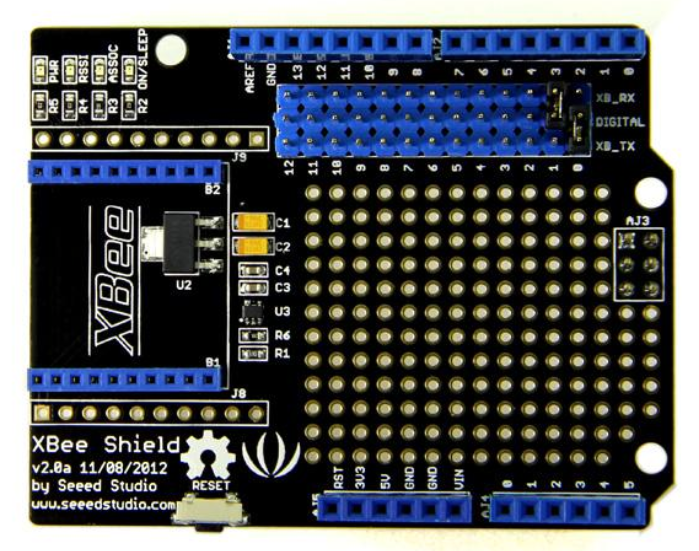
\includegraphics[width=0.55\textwidth]{figuras/EArte2.png}
\caption{XBee Shield v2.0 - Seeed Studio}
\label{fig:EArte2}
\end{figure}

Si se habla del lado de la Raspberry Pi, la interacción con el módulo XBee se realiza a través de una placa XBee Explorer.

Como uno puede comprobar, existe una gran variedad de placas y shields que adaptan y facilitan la interacción de los módulos XBee con las plataformas de ordenadores y microcontroladores más populares.

En este caso, los módulos XBee están configurados como AT. Más adelante en el documento se detalla esta cualidad.

\section{Smart Porch Light Project \cite{SPLP:MOUSER}}

En el contexto del Internet de las Cosas (IoT), el autor desarrolla un proyecto de red inalámbrica de sensores y actuadores sincronizados a una nube en la red.

El caso particular consta de una luz de exterior que es automáticamente controlada teniendo en cuenta los datos obtenidos de múltiples sensores que captan el estado del entorno. Estos sensores miden la luz ambiente, temperatura, humedad y luz ultravioleta. El control de la lámpara de exterior se lleva a cabo con un relé capaz de separar la etapa de potencia de la etapa de señal. Con el proyecto operativo, se usan servicios en la nube para almacenar y leer la información del estado del sistema; obteniendo como resultado una lámpara inteligente que permite mostrar a los usuarios el estado de los sensores desde cualquier dispositivo con acceso a internet.

Los componentes hardware, al ser todos del mismo fabricante (Seeed Studio), permiten su apilamento en un único stack compacto (figura \ref{fig:EArte4}) de microcontrolador, shields módulo XBee. El microcontrolador es un Arduino Mega, los shields son de sensores y de XBee y,coronando el stack, se encuentra el módulo XBee LTE.

\begin{figure}[t]
\centering
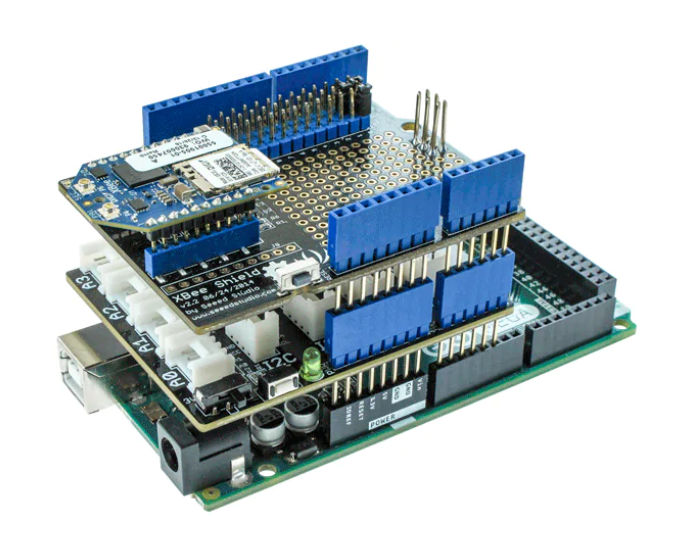
\includegraphics[width=0.55\textwidth]{figuras/EArte4.png}
\caption{Stack Hardware del proyecto 3.4}
\label{fig:EArte4}
\end{figure}

A diferencia de proyectos mencionados anteriormente, en este se usa una API REST en lugar de MQTT para transferir la información al servicio de nube correspondiente y los módulos XBee son del modelo LTE, por lo que pueden acceder a la red directamente sin la necesidad de poseer enlace alguno a un ordenador con conexión, bien vía USB o a través de otro módulo XBee. Por otro lado, la interfaz donde mostrar el estado de los sensores no se basa en Node-RED, sino en Ubidots.

\section{Home Automation System \cite{Molnar:Digi}}

Estamos ante otro proyecto del campo IoT que hace uso de módulos XBee. En este caso, los actuadores y sensores de una casa en la que se ha implementado este sistema domótico están conectados a red inalámbrica de módulos XBee mediante cableados como el que se muestra en la figura \ref{fig:EArte5}.

\begin{figure}[tb]
\centering
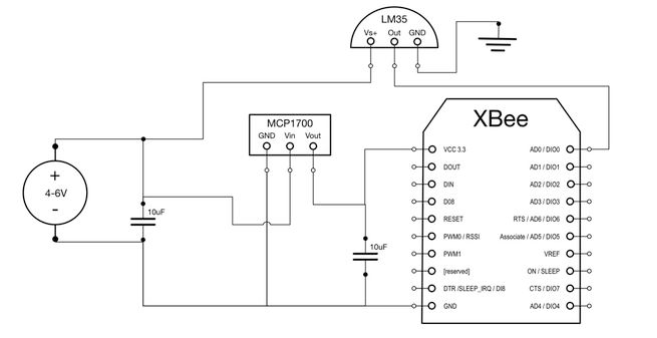
\includegraphics[width=0.55\textwidth]{figuras/EArte5.png}
\caption{Esquema de conexión del sensor de temperatura}
\label{fig:EArte5}
\end{figure}

La información se transmite a un portal central que tiene como base una placa Netduino o una Raspberry Pi con Windows IoT como sistema operativo. El portal envía y recibe mensajes de cada uno de los módulos XBee conectados y traduce la información de tal manera que el controlador lo pueda interpretar.

Usa MQTT para la comunicación controlador-portal pero recurre a una nueva herramienta, openHAB, para proporcionar una interfaz gráfica donde monitorizar y controlar los sensores y actuadores de la casa.

\section{Controlador central para un sistema domótico utilizando el protocolo inalámbrico ZigBee \cite{ULL:2016}}

Con este proyecto se habla del desarrollo de otro sistema domótico; esta vez basado en la placa de desarrollo Pandaboard (figura \ref{fig:EArte6}). A principios de la presente década, Pandaboard nació para competir en el mercado de los ordenadores pequeños de bajo coste, pero Raspberry terminó por dominar a la competencia. Hoy en día se trata de una placa obsoleta y poco usada por la comunidad.

\begin{figure}[tb]
\centering
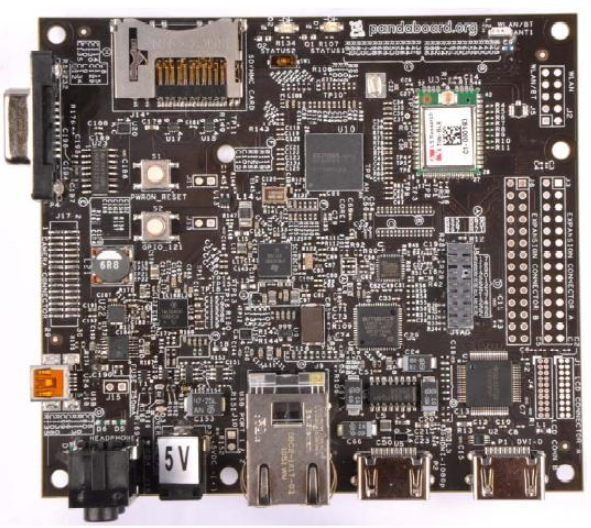
\includegraphics[width=0.55\textwidth]{figuras/EArte6.png}
\caption{PandaBoard ES}
\label{fig:EArte6}
\end{figure}

En este proyecto se recurre también al uso de dispositivos XBee para la transmisión de información y a MQTT. Incorpora Domoticz, un programa de supervisión y configuración domótica de código abierto.

Como particularidad de la que se hablará de manera mas detallada más adelante, en este caso los módulos XBee funcionan en configuración API, en contraposición al modo AT mencionado previamente en otro proyecto.

\section{Node-RED based custom full-room wake-up light \cite{Bulten:2019}}

Proyecto que desarrolla una aplicación Node-RED con el fin de configurar un patrón despertador configurable. El desarrollo del proyecto referenciado \cite{Bulten:2019} se centra en la definición de los flujos de Node-RED puesto que el sistema domótico se ha desarrollado previamente \cite{Bulten:2018}.

El flujo de Node-RED (figura \ref{fig:EArte7}) trabaja detectando la igualdad entre la hora programada y la actual. A continuación, comprueba si es fin de seamana y si está activada la alarma durante los fines de semana en la configuración. Por último y habiendo superado las etapas anteriores, se define una secuencia de iluminación de las bombillas correspondiente a la señal de despertador.

\begin{figure}[tb]
\centering
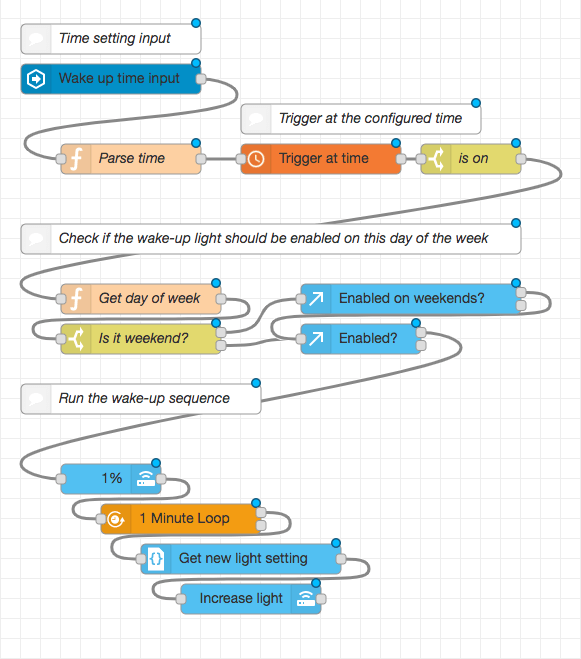
\includegraphics[width=0.75\textwidth]{figuras/EArte7.png}
\caption{Flujo de Node-RED}
\label{fig:EArte7}
\end{figure}

El proyecto domótico completo se basa en una instalación de Node-RED y Home Assistant, que proporciona la interfaz de usuario, sobre una Raspberry Pi. Las bombillas son bombillas inteligentes que reciben ordenes vía XBee. La recepción y envío de radiofrecuencia desde la Raspberry Pi se produce a través de un hub comercial que va alternando la conexión con las diferentes bombillas a muy alta velocidad.

\section{ArduSmartHome \cite{UOC:2017}}

El proyecto ArduSmartHome consiste en el desarrollo de un sistema domótico de control que capture datos del entorno a través de varios sensores y monitorizar esa información usando Node-RED.

La principal diferencia que tiene este proyecto con los mencionados previamente es la tecnología usada para la transmisión de la información. Mientras que hasta ahora se habiía usado principalmente radiofrecuencia a través de módulos XBee\footnote{La tecnología utilizada en el proyecto que describe este documento es, precisamente, radiofrecuencia usando módulos XBee}, en este caso se usa una red WiFi local.

\begin{figure}[tb]
\centering
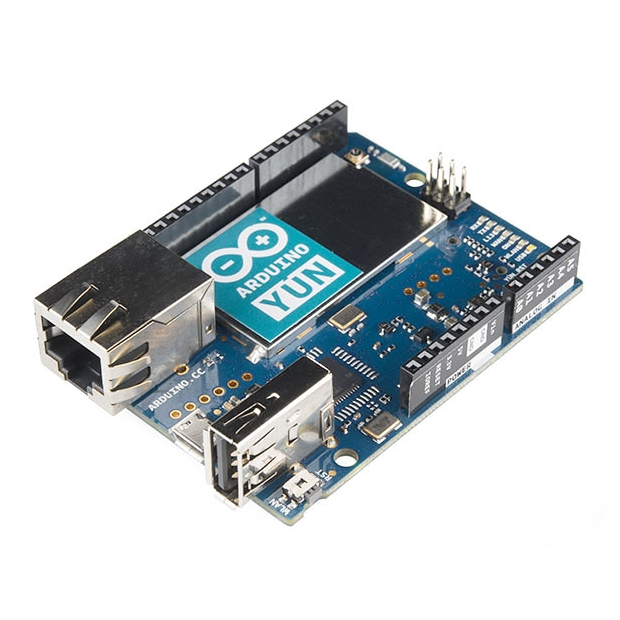
\includegraphics[width=0.55\textwidth]{figuras/EArte8.png}
\caption{Arduino Yun}
\label{fig:EArte8}
\end{figure}

Para conseguir esto, se hace uso de un microcontrolador diseñado para esta tarea, el Arduino Yun (figura \ref{fig:EArte8}). La red domótica posee varios de estos microcontroladores volcando los datos de los sensores que tienen conectados a la red local. Existe un Arduino Yun\footnote{Se puede lograr una equivalencia económica al Arduino Yun usando un Arduino UNO complementado con la shield de extensión Dragino Yun Shield v2.4} que ejerce las funciones de coordinador de las comunicaciones a la vez que es quién se encarga de establecerlas. En este proyecto también se hace uso de MQTT.

\section{University of Minnesota – Solar Vehicle \cite{UM:SV}}

Estudiantes de la Universidad de Minnesota llevan desde 1990 desarrollado prototipos de coches solares para competir en varios certámenes a nivel nacional e internacional, obteniendo grandes resultados. En este contexto, en 2019 se ha presentado el nuevo prototipo denominado EOS II (figura \ref{fig:EArte3}). 

\begin{figure}[b]
\centering
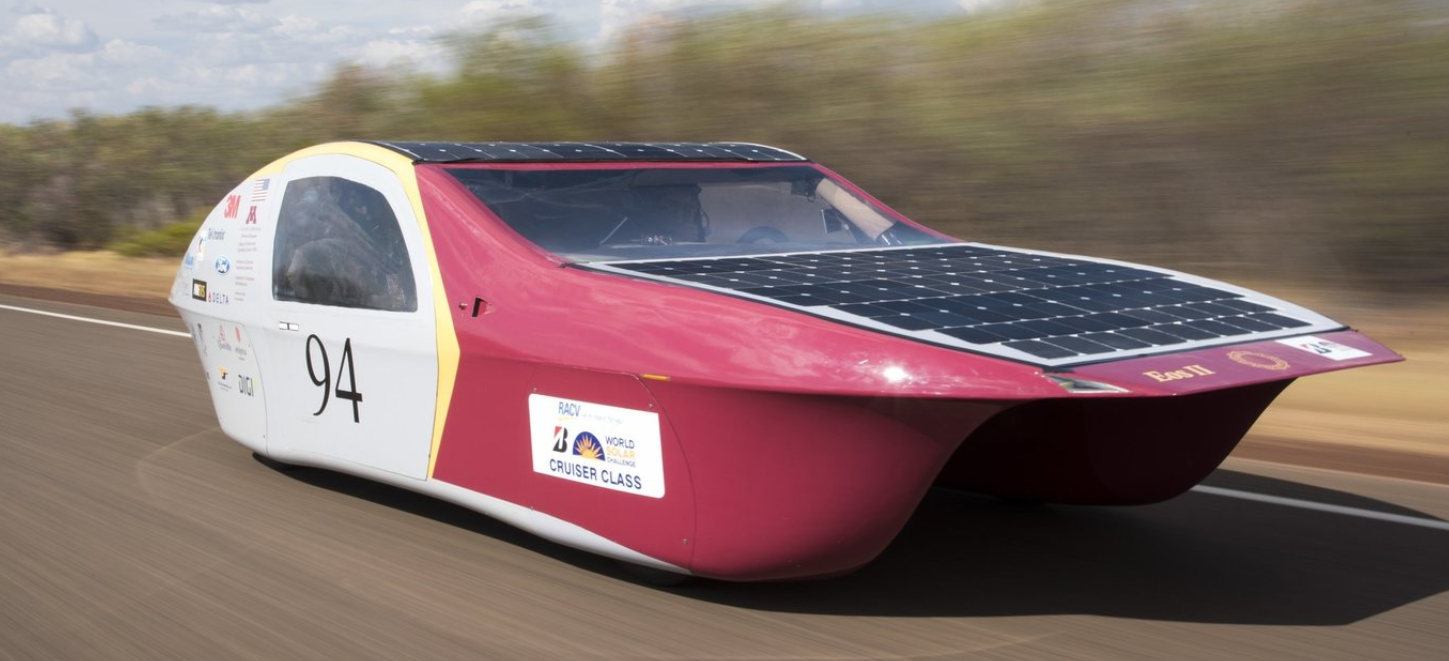
\includegraphics[width=0.55\textwidth]{figuras/EArte3.png}
\caption{EOS II Solar car}
\label{fig:EArte3}
\end{figure}

Con el apoyo de Digi, han implementado una red inalámbrica a la que conectan ordenadores y diferentes sensores. La conexión a esta red se realiza mediante módulos XBee. El objetivo final es la comunicación entre los módulos para la detección de errores y el almacenamiento de los datos adquiridos por esos mismos sensores durante el funcionamiento del prototipo.

\chapter{Cómo escribir en Latex}

\section{Estilo}

Al ser un documento científico-técnico, debe ser expuesto en tercera persona del singular. También se admite usar la primera persona cuando son apreciaciones personales del autor.

\section{Citas}

%las referencias a artículos se ponen con \cite, 
%las referencias a imágenes \ref, 
%y las referencias a ecuaciones \eqref

Esto es un ejemplo de cita de un artículo \cite{Brunete:2013}. Y este para una página web \cite{google2018}.

Se recomienda usar un archivo que contenga la bibliografía (.bibtex), aunque también se puede incluir la bibliografía directamente en el .tex mediante \verb=\bibitem=.


\section{Listas}

%itemize es una lista. Cada término lleva delante un \item
Ejemplo de lista de puntos:
\begin{itemize}
\item Ejemplo1.
\item Ejemplo2.
\end{itemize} 

Y lista numerada:
\begin{enumerate}
\item Elemento 1
\item Elemento 2
\end{enumerate}

\section{Tablas}

Ejemplo de tabla. Como se aprecia en la tabla \ref{tab:table_example}...
\begin{table}[tb]
\caption{Ejemplo de tabla}
\label{tab:table_example}
\begin{center}
\begin{tabular}{|c||c|c|}
\hline
One & Two & Three\\
\hline
\hline
F1A & F1B & F1C\\
F2A & F2B & F2C\\
\hline
\end{tabular}
\end{center}
\end{table}

\section{Referencia a una sección}
\label{sec:refsec}

Ejemplo de referencia a la sección \ref{sec:refsec}

\section{Texto}

Texto en \textbf{negrita} y \textit{cursiva}.

\section{Figuras}

Ejemplo de referencia a figura (figura \ref{fig:logo_upm}). Es importante que todas las figuras que aparezcan estén referenciadas, así como las tablas. En general las figuras se colocarán al principio o al final de cada página ([tb] en latex), a no ser que por alguna necesidad se deban colocar en una posición exacta ([h]).

%caption es el pie de foto, y label es el nombre que se da a la imagen para referenciarla después. label no puede llevar acentos y no se muestra de cara al documento final (es sólo interno).
\begin{figure}[tb]
\centering

\includegraphics[width=0.45\textwidth]{figuras/Logo_UPM.jpg}   
\caption{Logotipo de la UPM}
\label{fig:logo_upm}
\end{figure}

\textbf{Muy importante!: Todas las figuras no originales que aparezcan en la memoria deben ir referenciadas.}


\section{Código software}

Existen muchas formas de escribir código en el TFG. Aquí se muestra una de ellas. En general es interesante numerar las líneas para que sean referenciables y destacar palabras clave del lenguaje correspondiente. Ver código \ref{code:prog1}.

% Esto para configurar como se va a visualizar el código
\lstset{numbers=left,numberstyle=\tiny, language=C, breaklines=true, basicstyle=\footnotesize, xleftmargin=25pt, framesep=8pt, numbersep=15pt}


\begin{lstlisting}[frame=leftline, caption={Hola Mundo}, label=code:prog1]
#include <iostream> 

using namespace std;

int main(int argc, char *argv[]) {
  cout << ``Hola mundo'' << endl;
  return 0;
}
\end{lstlisting}


En general no se debe incluir mucho código en la memoria. El código debe ir en el Anexo. 

\section{Pie de página}

Esto es un pie de página \footnote{Pie de página}. Y para usar direcciones web y no tener problemas con caracteres especiales (como el ``\_''), se usa el comando url \footnote{\url{https://es.wikipedia.org/wiki/Estado_del_arte}}


\chapter{Resultados y discusión}

En este capítulo...


\section{Resultados}

Los resultados son una parte imprescindible del TFG. Muestran lo que realmente se ha hecho y deben ser explicados con rigor y claridad

\subsection{Test User Interface}

\subsection{Test MQTT}


\section{Discusión}

Una vez expuestos los resultados en la sección anterior, aquí se deben comentar y analizar su validez.

\chapter{Gestión del proyecto}

En este capítulo se describe la gestión del proyecto: ciclo de vida, planificación, presupuesto, etc.

\section{Ciclo de vida}

Explicación de las fases del proyecto: definición, análisis, diseño, construcción, pruebas, implementación, validación, documentación. Ejemplo: diagrama de Pert.

\section{Planificación}

Se puede indicar mediante un diagram de Gantt.

\subsection{Planificación inicial}

\subsection{Planificación final}


\section{Presupuesto}

\subsection{Personal}

\subsection{Material}

\subsection{Resumen de costes}

\chapter{Conclusiones}

Se presentan, a continuación, las conclusiones sacadas del desarrollo del proyecto, así como se proponen futuros desarrollos relacionados con las tecnologías trabajadas.

\section{Conclusión}

Alcanzado este punto, cabe revisar lo obtenido para hacer una valoración global de lo que ha supuesto el proyecto. 

Como resumen, se han alcanzado todos los objetivos fijados al inicio gracias a un proceso de aprendizaje por varios frentes que ha culminado en una integración limpia y funcional del brazo robótico RoboHealth Arm en la red domótica existente. Desde el comienzo, las características del proyecto hacían ver que el trabajo se iba a repartir de manera modular para tratar de coordinar la distintas tecnologías presentes.

XBee como soporte para la tecnología de radiofrecuencia ha resultado ser una solución realmente interesante por las facilidades que aporta tanto para trabajar con ello, como para usarlo de manera integrada. Hace unos años, Digi renovó su interfaz de configuración XCTU y ha dado un empujón muy interesante a todos sus productos XBee. Existe una comunidad grande y activa centrada en estos módulos y su gran catálogo los convierten en una de las mejores soluciones inalámbricas a día de hoy.

Este proyecto ha contribuido al compendio de trabajos que se aglutinan en torno al proyecto RoboHealth y ahora un nuevo elemento se une a su red domótica, quizás el que más utilidad podría aportar a día de hoy a un supuesto paciente al que ofrecer toda esta tecnología. Un brazo robótico, usado de una manera inteligente, puede ofrecer multitud de posibilidades debido a su versatilidad.

\section{Desarrollos futuros}

Si bien por el lado de este proyecto se está llegando a un límite de desarrollo, existen varias propuestas que podrían desarrollarse en un futuro:

\begin{itemize}
\item La rehabilitación y actualización en una segunda revisión de RoboHealth Arm daría aún más utilidad a su integración en la red. Actualmente, RHA tiene el eje Z inutilizado y sería planteable su rehabilitación, así como el propio brazo en su conjunto podría admitir mejoras en su funcionamiento. Alguna de estas mejoras podría ser la inclusión de actuadores de señalización o iluminación, alarmas, etc; con el fin de aumentar las funcionalidades más allá del uso de la tablet para la que está concebida. Otra posibilidad es añadir un grado de libertad al robot, permitiéndole regular la orientación de la tablet haciendo uso de un servomotor.

\item La inclusión de RHA en la lista de dispositivos que responden al topic MQTT de la habitación hace que se integre en un sistema que puede ser utilizado para múltiples objetivos. Uno de ellos puede ser el desarrollo de un programa que coordine todos los dispositivos a través de MQTT. De esta manera, se pueden generar recetas que aplicar bajo ciertos condicionantes. A cierta hora, subir las persianas, subir la cama y disponer la tablet al paciente; por ejemplo.

\item La inclusión de nuevos elementos a la red MQTT podría proporcionar más usos a RHA. Por ejemplo, existe la posibilidad de comandar hablando el brazo robótico si se integra un sistema de reconocimiento de voz.

\end{itemize}

\appendix

\chapter{Anexo A}

El Anexo A recoge y explica los procesos de instalación y configuración de los diferentes sistemas operativos, programas y herramientas necesarios para la implementación del proyecto.

% Configuración de la visualización del código SW
\lstset{backgroundcolor=\color{verde_p}, language=bash, breaklines=true, basicstyle=\footnotesize, xleftmargin=25pt, framesep=8pt, numbersep=15pt}


\section{Instalación de Raspbian OS}\label{anexo:raspbian}

Raspbian es un sistema operativo orientado a Raspberry Pi por lo que existe multitud de documentación complementaria en la web oficial\cite{Raspberry:2019}

Antes de comenzar a instalar el sistema operativo en una tarjeta microSD, se debe comprobar que ésta reúne los requisitos para ser usada en esta aplicación. Uno de estos requisitos es que la capacidad de la tarjeta sea superior a 8GB. Sin embargo, el uso de tarjetas de un tamaño superior a 32GB hace que sea necesario formatear la tarjeta antes de instalar el sistema operativo. Esto es debido a que el formato de serie (exFAT) no es compatible con el bootloader de Raspberry Pi, por lo que se deberá aplicar el formato FAT16 o FAT32 previamente.

Las instrucciones están pensadas teniendo en cuenta que se posee un ordenador con sistema operativo Windows.

\begin{enumerate}
\item \textbf{Descargar el sistema operativo}

Se puede descargar la imagen desde la web de descargas de Raspberry Pi\footnote{\url{https://www.raspberrypi.org/downloads/raspbian/}}

\begin{figure}[tb]
\centering

\includegraphics[width=0.5\textwidth]{figuras/RaspbianDwIcon.png}
\caption{Descarga de Raspbian Stretch}
\label{fig:descargaRaspbian}
\end{figure}

\item \textbf{Descargar e instalar Etcher}

Se precisa de una herramienta de escritura de imágenes y Etcher es la solución más sencilla para la mayoría de usuarios. Permite la escritura de la imagen sin la necesidad de extraer el archivo zip. 


\item \textbf{Escribir la imagen a una microSD}

Seleccionar el archivo de la imagen  la SD de destino es suficiente para flashear la imagen.

\item Una vez acabado el proceso de descompresión, la instalación debería estar completada. Introduciendo la tarjeta micro SD en su correspondiente posición en la Raspberry Pi, ésta acederá a Raspbian para arrancar el sistema.

\item Para comprobar la version del SO instalado, se puede hacer uso del comando \textit{lsb-release}

\begin{lstlisting}[frame=single, label=command:lsb]
lsb_release -a
\end{lstlisting}

\begin{figure}[tb]
\centering
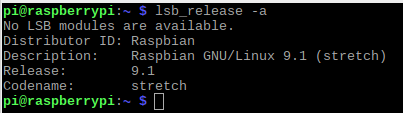
\includegraphics[width=0.5\textwidth]{figuras/RaspbianVersion.png}
\caption{Versión de Raspbian}
\label{fig:versionRaspbian}
\end{figure}

\end{enumerate}


\section{Instalación MQTT en Raspbian OS}\label{anexo:mqtt}

Mosquitto (broker de MQTT) se instala de igual manera que cualquier otra aplicación, haciendo uso de los repositorios.

En primer lugar, se actualizan los repositorios.

\begin{lstlisting}[frame=single, label=command:installmqtt1]
sudo apt-get update
\end{lstlisting}

Posteriormente, se instala Mosquitto.

\begin{lstlisting}[frame=single, label=command:installmqtt2]
sudo apt-get install mosquitto
\end{lstlisting}

Si todo va bien, al terminar el proceso, MQTT debería estar instalado.

Para probar la instalación, se pueden usar clientes de MQTT para enviar y recibir información a través un topic de prueba. Estos clientes son, por ejemplo, \textit{IoT MQTT Dashboard} en Android o \textit{MQTT.fx} en Windows.

\section{Edición y compilación de scripts en Raspbian OS}



\chapter{Anexo B}

En el Anexo B se sitúan los desarrollos software íntegros que forman parte del proyecto.

\section{Código SendAT.py}

\section{Código SendAPI.py}

\section{Código Receive.py}


\chapter{Anexo C}

El Anexo C recoge la documentación de interés de distintos componentes del proyecto

\section{Datasheet XBee Shield}

\backmatter
%Glosario, lista de símbolos, notas, etc.

%estilo de bibliografía: plana, alfa...
\bibliographystyle{plain}

%genera doble hoja en blanco
\cleardoublepage

%apartado de bibliografía
\addcontentsline{toc}{chapter}{Bibliografia}

%se incluye la bibliografía. Archivo de tipo .bib (bibtex)
\bibliography{bibliografia/bibliografia}

%fin del documento
\end{document}